\section{量子线路实现}
本文采用 $4$ qubits 参数化量子特征映射电路。对每个局地窗口特征，先通过 Hadamard 门与单比特旋转门建立基本编码，再使用相邻量子比特之间的受控相位和旋转门刻画局地分量之间的耦合关系。该设计具有两点优势：其一，线路规模固定、资源开销低，满足赛题比特限制；其二，线路表达的是局地几何关系，便于与 LETKF 的局地分析思想对应。

量子相似度由量子态重叠直接给出，不需要额外训练大型量子模型，因此实现简单且可复现。当前方案中单次量子线路仅使用 $4$ 个量子比特，远低于赛题规定的 $30$ qubits 上限。

\begin{figure}[htbp]
\centering
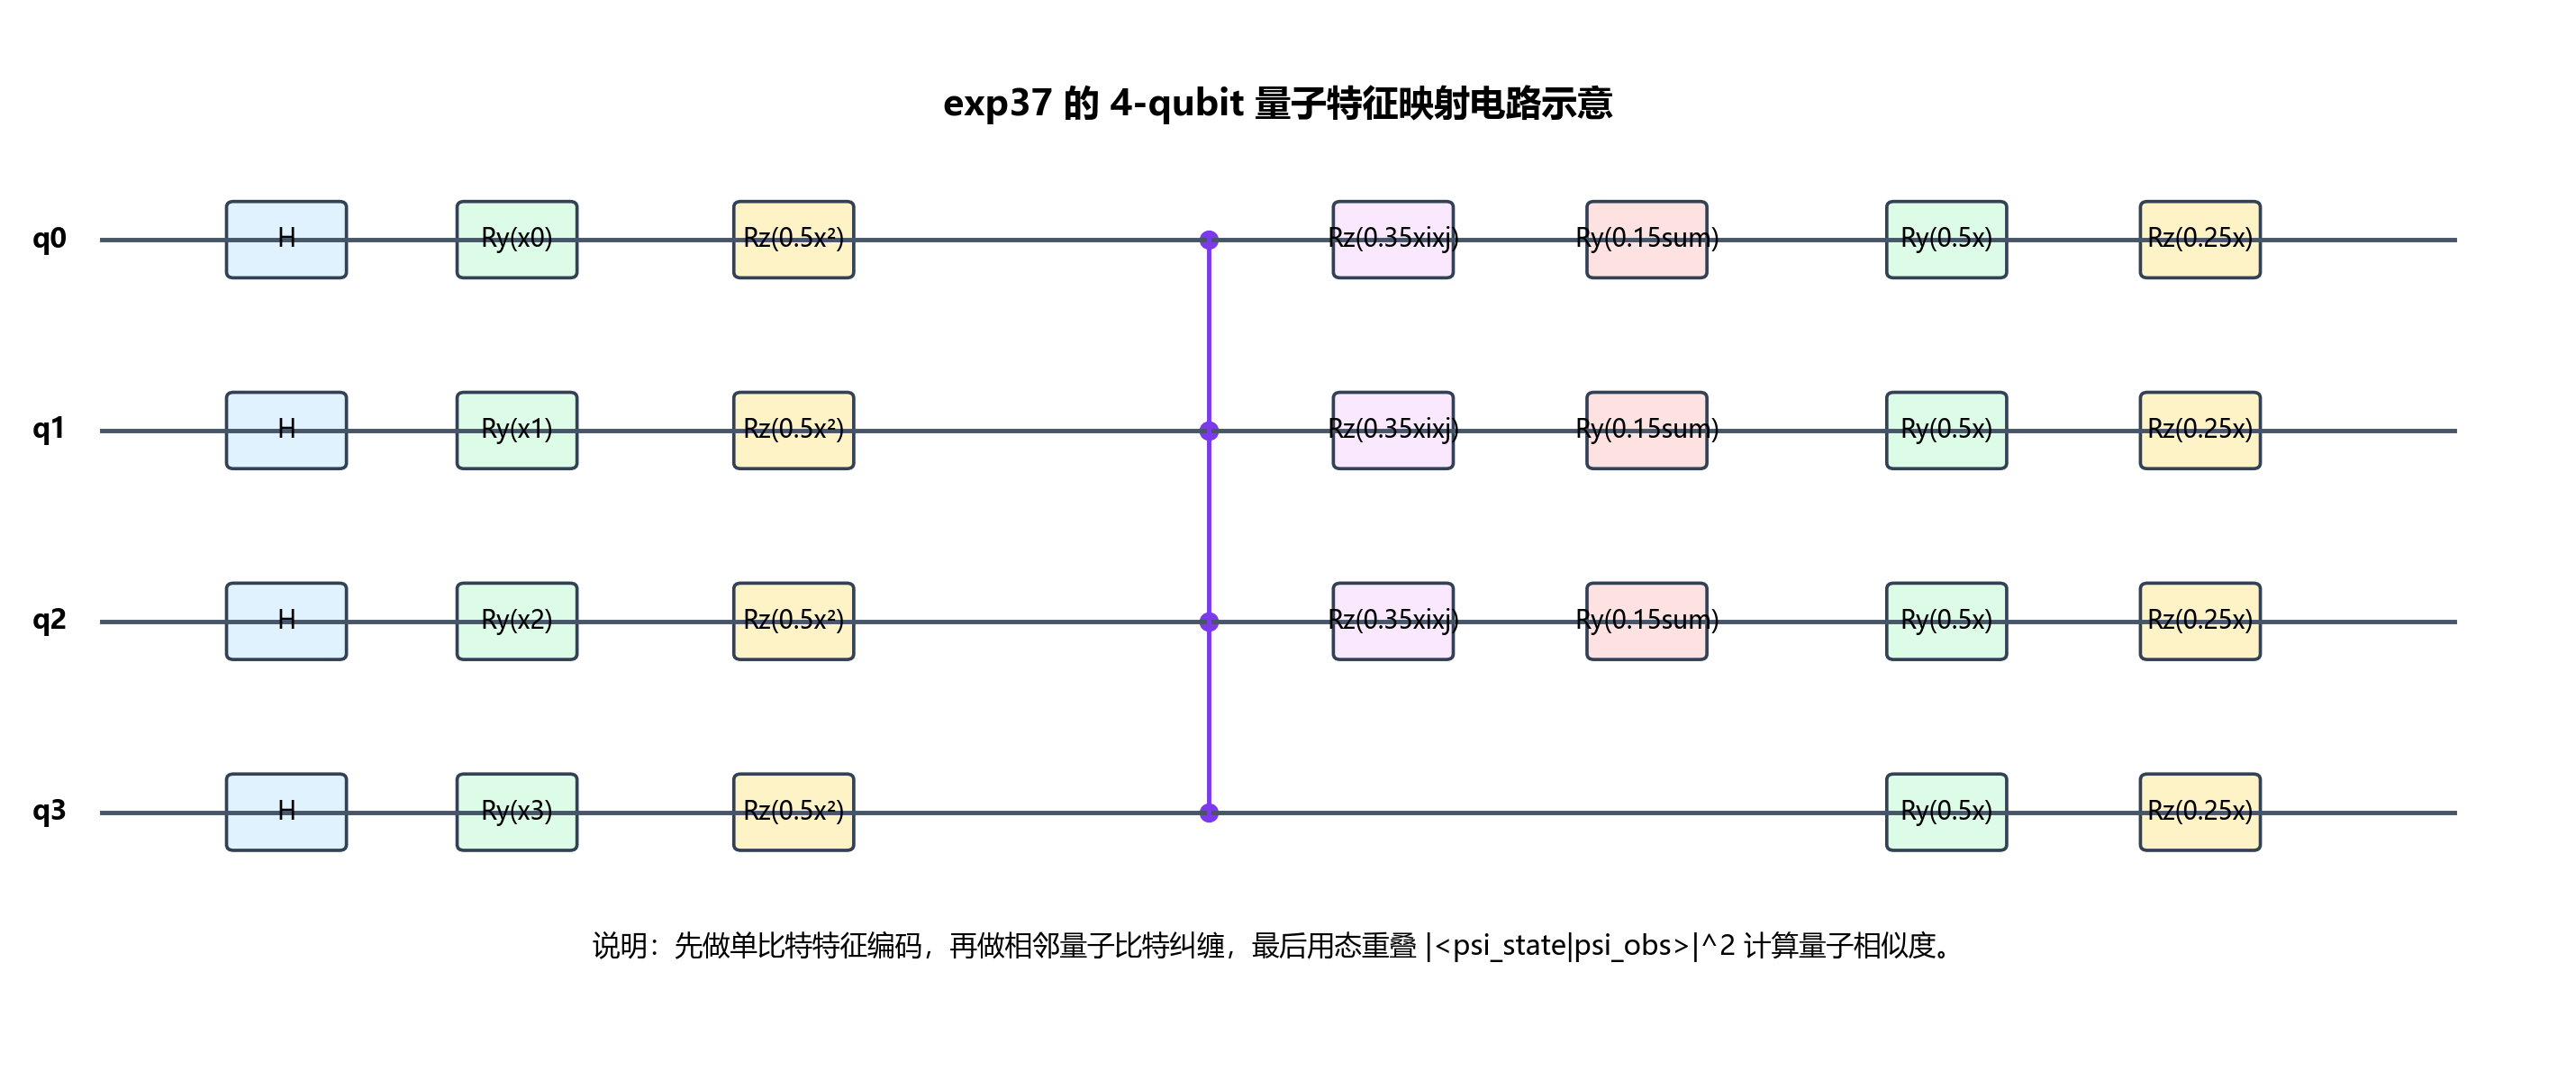
\includegraphics[width=0.82\linewidth]{figures/exp37_quantum_circuit_schematic.png}
\caption{4-qubit 量子特征映射电路示意。}
\label{fig:circuit}
\end{figure}

图 \ref{fig:circuit} 表明当前方案只使用 $4$ qubits 的浅层线路即可完成局地结构编码，因此在资源层面具有明显优势。与需要更深层电路或更大量子比特的方案相比，这种实现更适合在受限模拟环境中稳定运行，也更容易解释不同门结构对局地模式表达的作用。

更重要的是，图 \ref{fig:circuit} 使“可解释性”不再停留在算法层面，而落实到了线路层面。线路前半部分的单比特编码负责把局地窗口中的数值特征转入量子态，后半部分的相邻耦合门则负责表达局地分量之间的关系。这意味着本文并不是任意选了一条量子线路来满足赛题要求，而是让线路结构与局地几何建模目标保持一致。也正因为电路浅、结构清晰，我们才有可能把后续的量子相似度矩阵、权重变化和 $J$ 修正联系起来做解释。

\begin{figure}[htbp]
\centering
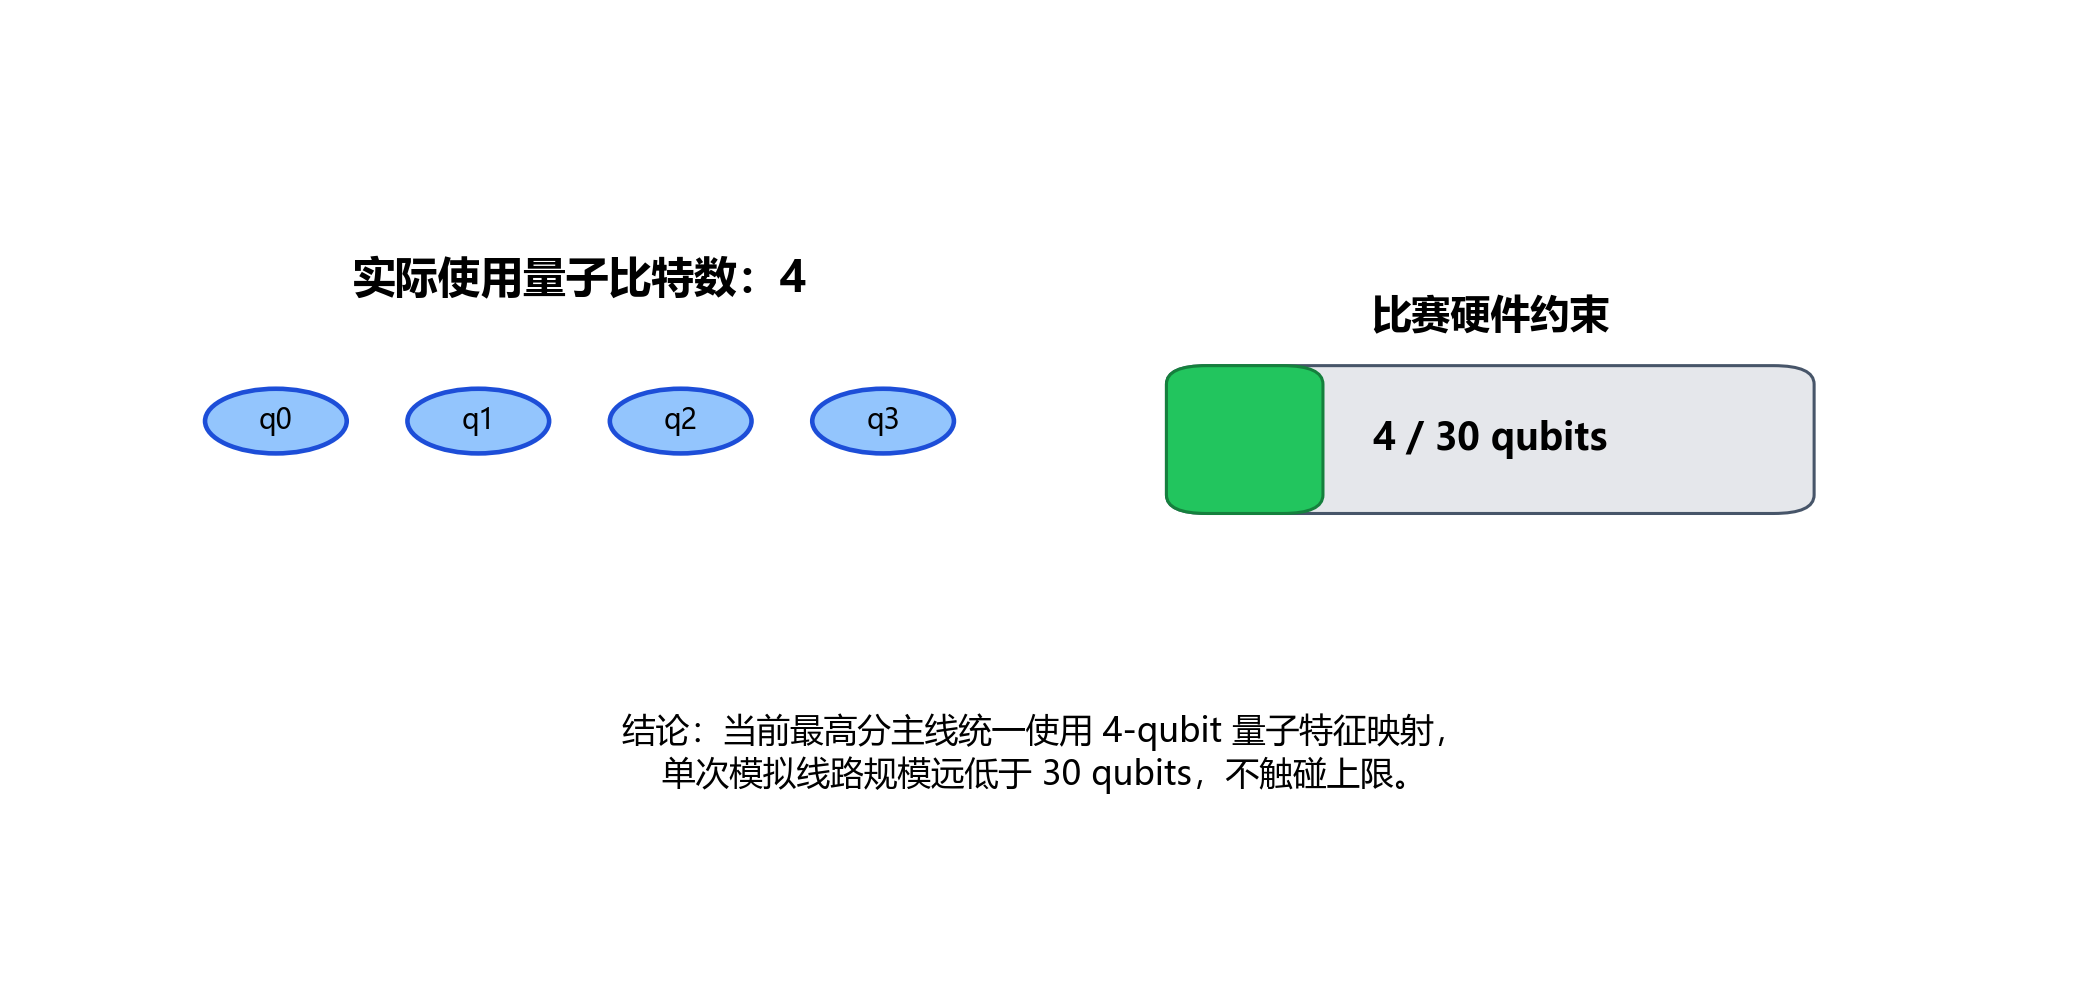
\includegraphics[width=0.88\linewidth]{figures/quantum_qubit_compliance.png}
\caption{当前方案的量子比特使用量与赛题上限对比。}
\label{fig:qubits}
\end{figure}

图 \ref{fig:qubits} 则从资源合规性的角度补充了另一层说明。当前方案仅使用 $4$ qubits，远低于赛题要求的 $30$ qubits 上限，这说明本文并不是依赖大规模量子资源“堆”出结果，而是在严格受限的线路规模下，通过局地建模与结构化融合获得增益。对评委而言，这一点非常关键，因为它证明方案具有真实的工程可实施性，而不是只在理想化资源条件下成立。

从整体上看，本节两张图分别回答了两个问题：图 \ref{fig:circuit} 回答“线路是怎么工作的”，图 \ref{fig:qubits} 回答“线路为什么合规且现实可行”。前者支撑可解释性，后者支撑工程可交付性。两者结合，才能完整说明本文所采用的量子线路不仅存在，而且是为本任务量身设计、可以实际运行且便于分析的。
